% =====================================================================
%  Capítulo 10 — Tipos de agresiones
% =====================================================================
\chapter{Tipos de agresiones}
\citacap{Quien conoce el peligro aprende a evitarlo.}{Proverbio}

El agresor puede interactuar con nosotras de las siguientes formas:

\begin{enumerate}
  \item Golpes con la mano dominante (diestra o zurda), con o sin agarre de la otra.
  \item Golpes con ambas manos: alternos o aleatorios.
  \item Golpes que no llegan a impactar, en muchas ocasiones desequilibrando al agresor (por buen movimiento de la agredida o error de cálculo del agresor).
  \item Golpes que impactan, llevando a doblegarse o caer al suelo.
  \item Agarres, con tres posibilidades: \textbf{(a)} agarre que busca trasladarme a un sitio donde no quiero ir ---de un agarre pasará a otro hasta cambiar la dinámica---; \textbf{(b)} agarre que busca que me quede estática, muchas veces golpeando con la otra mano; \textbf{(c)} agarre intimidatorio, para recortar distancia y amenazar con superioridad física.
\end{enumerate}

\begin{reglaoro}
\textbf{Contra el traslado:} nunca dejarse llevar a un \enquote{segundo lugar} (un coche, un portal, un descampado). Las estadísticas policiales coinciden: el segundo lugar siempre es peor que el primero, porque es el terreno elegido por el agresor. Resiste, grita y lucha en el primer escenario, donde aún hay testigos posibles.
\end{reglaoro}

\newpage

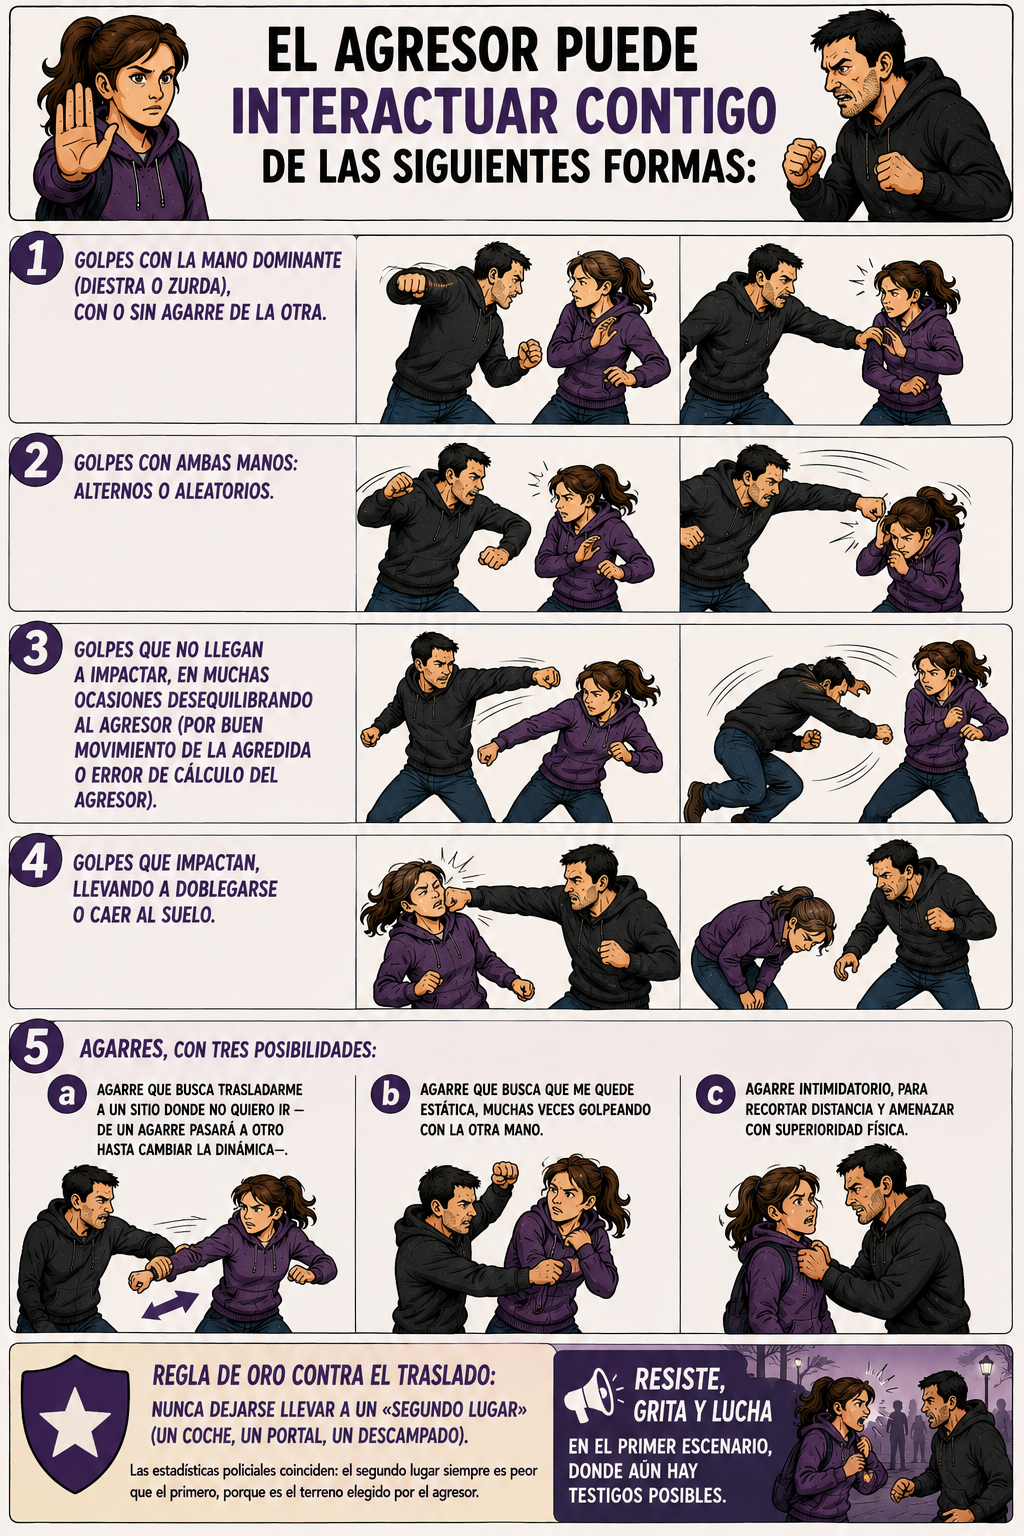
\includegraphics[width=\linewidth]{figures/tipos-agresiones.png}